\chapter{What Are Symbols?}
\label{ch:symbols}

\begin{nontechnical}
\textbf{A symbol is like a ``word'' in radio language}---instead of sending individual letters (bits), you send whole words (symbols) to go faster!

\textbf{Simple analogy: Semaphore flags}
\begin{itemize}
\item \textbf{Bit-by-bit:} Flag up = 1, flag down = 0. Message ``HI'' (8 bits) = 8 flag movements
\item \textbf{Symbol-by-symbol:} Four flag positions = 1 symbol = 2 bits each!
  \begin{itemize}
  \item Up-right = ``00'', Up-left = ``01'', Down-left = ``10'', Down-right = ``11''
  \item Same message takes only 4 movements = \textbf{2$\times$ faster!}
  \end{itemize}
\end{itemize}

\textbf{Real modulation examples:}
\begin{itemize}
\item BPSK: 1 bit/symbol (like a light switch: on/off)
\item QPSK: 2 bits/symbol (like a 4-way hand gesture)
\item 16-QAM: 4 bits/symbol (like showing fingers 0--15)
\item 256-QAM: 8 bits/symbol (like sign language with 256 distinct signs)
\end{itemize}

\textbf{Why it matters:} Your phone switches between modulations. Strong signal $\rightarrow$ 256-QAM (8 bits/symbol, fast!). Weak signal $\rightarrow$ BPSK (1 bit/symbol, reliable!). That's an 8$\times$ speed difference.
\end{nontechnical}

\section{Overview}

In digital communication, a \textbf{symbol} is a fundamental unit of information transmitted over the channel during one signaling interval. A symbol represents a group of bits that are mapped to a unique signal state (amplitude, phase, frequency, or combination thereof).

\begin{keyconcept}
\textbf{Symbols enable bandwidth-efficient communication.} By encoding multiple bits per symbol (e.g., QPSK: 2 bits/symbol, 16-QAM: 4 bits/symbol), we transmit more information within the same bandwidth, effectively multiplying data throughput without increasing occupied spectrum.
\end{keyconcept}

\section{Mathematical Definition}

\subsection{Bit Rate and Symbol Rate}

The relationship between bit rate and symbol rate is fundamental:
\begin{equation}
R_b = R_s \cdot m
\end{equation}
where:
\begin{itemize}
\item $R_b$ = bit rate (bits per second, bps)
\item $R_s$ = symbol rate (symbols per second, baud)
\item $m$ = number of bits per symbol (dimensionless)
\end{itemize}

\textbf{Alternative expression:}
\begin{equation}
m = \log_2(M)
\end{equation}
where $M$ is the number of distinct symbols (constellation size).

\subsection{Symbol Duration}

The symbol period $T_s$ is the time allocated to transmit one symbol:
\begin{equation}
T_s = \frac{1}{R_s} = \frac{m}{R_b}
\end{equation}

For $m$ bits per symbol, the bit period is:
\begin{equation}
T_b = \frac{T_s}{m} = \frac{1}{R_b}
\end{equation}

\begin{calloutbox}{Example: QPSK System}
\begin{itemize}
\item Data rate: $R_b = 1$ Mbps
\item Modulation: QPSK ($m = 2$ bits/symbol)
\item Symbol rate: $R_s = R_b / m = 1/2 = 500$ ksps (kilosymbols/sec)
\item Symbol period: $T_s = 1/R_s = 2$ µs
\item Bit period: $T_b = 1/R_b = 1$ µs
\end{itemize}

\textbf{Result:} Each symbol lasts 2~µs and carries 2~bits of information.
\end{calloutbox}

\section{Symbol Mapping and Constellations}

\subsection{From Bits to Symbols}

The process of converting binary data to symbols involves \textbf{grouping} and \textbf{mapping}:

\begin{center}
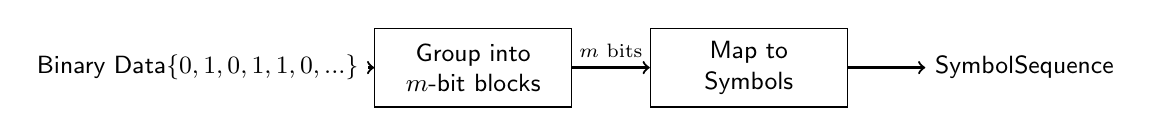
\begin{tikzpicture}[
  block/.style={rectangle, draw, minimum width=2.5cm, minimum height=1cm, font=\sffamily\small, align=center},
  node distance=2.5cm,
  font=\small
]
\node (bits) {\sffamily Binary Data\\$\{0, 1, 0, 1, 1, 0, ...\}$};
\node[block, right of=bits, node distance=3.5cm] (group) {Group into\\$m$-bit blocks};
\node[block, right of=group, node distance=3.5cm] (map) {Map to\\Symbols};
\node[right of=map, node distance=3.5cm] (symbols) {\sffamily Symbol\\Sequence};

\draw[->,thick] (bits) -- (group);
\draw[->,thick] (group) -- node[above,font=\scriptsize] {$m$ bits} (map);
\draw[->,thick] (map) -- (symbols);
\end{tikzpicture}
\end{center}

\textbf{Example: QPSK (2 bits/symbol)}

Binary stream: \texttt{0 0 1 1 0 1 1 0}

\begin{enumerate}
\item \textbf{Group:} \texttt{00}, \texttt{11}, \texttt{01}, \texttt{10}
\item \textbf{Map to symbols:}
  \begin{itemize}
  \item \texttt{00} $\rightarrow$ Symbol $s_0$ (phase $45°$)
  \item \texttt{11} $\rightarrow$ Symbol $s_3$ (phase $225°$)
  \item \texttt{01} $\rightarrow$ Symbol $s_1$ (phase $135°$)
  \item \texttt{10} $\rightarrow$ Symbol $s_2$ (phase $315°$)
  \end{itemize}
\item \textbf{Transmit:} 4 symbols instead of 8 individual bits
\end{enumerate}

\subsection{Constellation Diagrams}

A \textbf{constellation diagram} is an IQ-plane visualization showing all possible symbol states:

\begin{center}
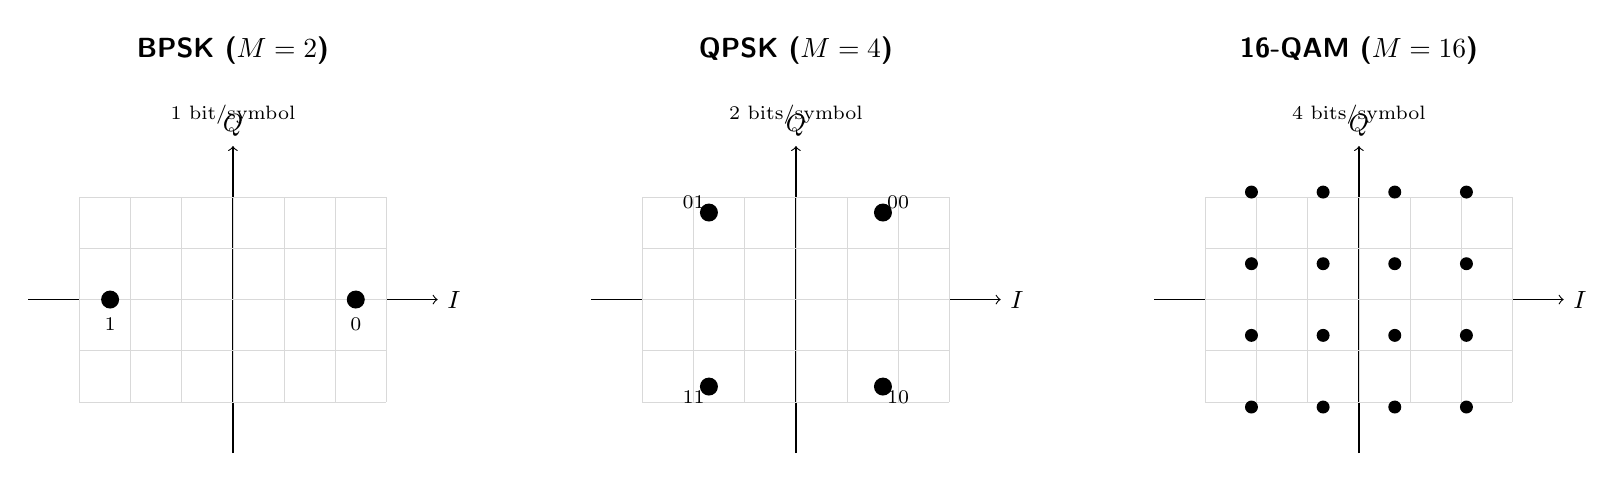
\begin{tikzpicture}[scale=1.3]
% BPSK (2 symbols)
\begin{scope}[shift={(0,0)}]
\node[above,font=\sffamily\bfseries] at (0,2.2) {BPSK ($M=2$)};
\node[below,font=\scriptsize] at (0,2) {1 bit/symbol};
\draw[->] (-2,0) -- (2,0) node[right,font=\sffamily\small] {$I$};
\draw[->] (0,-1.5) -- (0,1.5) node[above,font=\sffamily\small] {$Q$};
\draw[very thin,gray!30] (-1.5,-1) grid[step=0.5] (1.5,1);
\fill[black] (-1.2,0) circle (2.5pt);
\fill[black] (1.2,0) circle (2.5pt);
\node[below=3pt,font=\scriptsize] at (-1.2,0) {1};
\node[below=3pt,font=\scriptsize] at (1.2,0) {0};
\end{scope}

% QPSK (4 symbols)
\begin{scope}[shift={(5.5,0)}]
\node[above,font=\sffamily\bfseries] at (0,2.2) {QPSK ($M=4$)};
\node[below,font=\scriptsize] at (0,2) {2 bits/symbol};
\draw[->] (-2,0) -- (2,0) node[right,font=\sffamily\small] {$I$};
\draw[->] (0,-1.5) -- (0,1.5) node[above,font=\sffamily\small] {$Q$};
\draw[very thin,gray!30] (-1.5,-1) grid[step=0.5] (1.5,1);
\fill[black] (0.85,0.85) circle (2.5pt);
\fill[black] (-0.85,0.85) circle (2.5pt);
\fill[black] (-0.85,-0.85) circle (2.5pt);
\fill[black] (0.85,-0.85) circle (2.5pt);
\node[above right=-2pt,font=\scriptsize] at (0.85,0.85) {00};
\node[above left=-2pt,font=\scriptsize] at (-0.85,0.85) {01};
\node[below left=-2pt,font=\scriptsize] at (-0.85,-0.85) {11};
\node[below right=-2pt,font=\scriptsize] at (0.85,-0.85) {10};
\end{scope}

% 16-QAM (16 symbols)
\begin{scope}[shift={(11,0)}]
\node[above,font=\sffamily\bfseries] at (0,2.2) {16-QAM ($M=16$)};
\node[below,font=\scriptsize] at (0,2) {4 bits/symbol};
\draw[->] (-2,0) -- (2,0) node[right,font=\sffamily\small] {$I$};
\draw[->] (0,-1.5) -- (0,1.5) node[above,font=\sffamily\small] {$Q$};
\draw[very thin,gray!30] (-1.5,-1) grid[step=0.5] (1.5,1);
% 16-QAM grid
\foreach \x in {-1.05,-0.35,0.35,1.05}
  \foreach \y in {-1.05,-0.35,0.35,1.05}
    \fill[black] (\x,\y) circle (1.8pt);
\end{scope}
\end{tikzpicture}
\end{center}

\textbf{Key observations:}
\begin{itemize}
\item More constellation points $\rightarrow$ more bits per symbol $\rightarrow$ higher data rate
\item Points closer together $\rightarrow$ more susceptible to noise
\item Euclidean distance between points determines noise immunity
\end{itemize}

\section{Gray Coding}

To minimize bit errors when symbols are corrupted by noise, we use \textbf{Gray coding}: adjacent symbols differ by only \textbf{one bit}.

\subsection{QPSK Gray Code Example}

\begin{center}
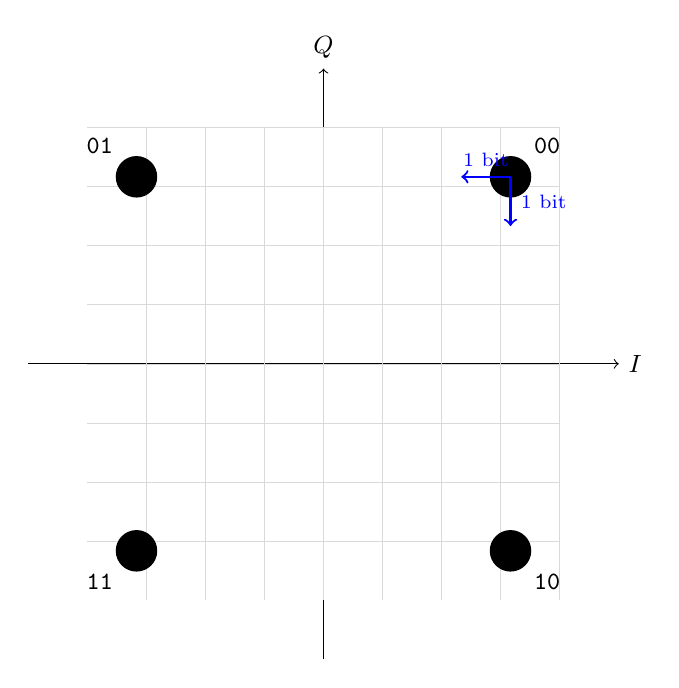
\begin{tikzpicture}[scale=2.5]
\draw[->] (-1.5,0) -- (1.5,0) node[right,font=\sffamily\small] {$I$};
\draw[->] (0,-1.5) -- (0,1.5) node[above,font=\sffamily\small] {$Q$};
\draw[very thin,gray!30] (-1.2,-1.2) grid[step=0.3] (1.2,1.2);

% QPSK constellation with Gray coding
\fill[black] (0.95,0.95) circle (3pt);
\fill[black] (-0.95,0.95) circle (3pt);
\fill[black] (-0.95,-0.95) circle (3pt);
\fill[black] (0.95,-0.95) circle (3pt);

% Labels with Gray code
\node[above right=5pt,font=\small\bfseries] at (0.95,0.95) {\texttt{00}};
\node[above left=5pt,font=\small\bfseries] at (-0.95,0.95) {\texttt{01}};
\node[below left=5pt,font=\small\bfseries] at (-0.95,-0.95) {\texttt{11}};
\node[below right=5pt,font=\small\bfseries] at (0.95,-0.95) {\texttt{10}};

% Show adjacent differences
\draw[->,thick,blue] (0.95,0.95) -- (0.7,0.95) node[midway,above,font=\scriptsize] {1 bit};
\draw[->,thick,blue] (0.95,0.95) -- (0.95,0.7) node[midway,right,font=\scriptsize] {1 bit};
\end{tikzpicture}
\end{center}

\textbf{Benefit:} If noise causes a symbol error to the nearest neighbor, only \textbf{one bit} is wrong, not multiple bits.

\textbf{Without Gray coding} (natural binary):
\begin{itemize}
\item \texttt{00} $\leftrightarrow$ \texttt{11}: 2-bit difference (poor)
\end{itemize}

\textbf{With Gray coding:}
\begin{itemize}
\item \texttt{00} $\leftrightarrow$ \texttt{01}: 1-bit difference (optimal)
\item \texttt{00} $\leftrightarrow$ \texttt{10}: 1-bit difference (optimal)
\end{itemize}

\section{Spectral Efficiency}

\subsection{Bits Per Symbol and Bandwidth}

The key advantage of symbols: \textbf{increase data rate without increasing bandwidth}.

\textbf{Shannon-Hartley capacity:}
\begin{equation}
C = B \log_2(1 + \text{SNR})
\end{equation}
where:
\begin{itemize}
\item $C$ = channel capacity (bps)
\item $B$ = bandwidth (Hz)
\item SNR = signal-to-noise ratio (linear, not dB)
\end{itemize}

\textbf{Spectral efficiency} $\eta$ measures how efficiently we use bandwidth:
\begin{equation}
\eta = \frac{R_b}{B} = \frac{R_s \cdot m}{B} \quad \text{(bps/Hz)}
\end{equation}

\begin{center}
\begin{tabular}{@{}lccr@{}}
\toprule
Modulation & $m$ (bits/symbol) & $M$ (states) & $\eta$ (bps/Hz) \\
\midrule
BPSK & 1 & 2 & 0.7--1.0 \\
QPSK & 2 & 4 & 1.4--2.0 \\
8PSK & 3 & 8 & 2.1--3.0 \\
16-QAM & 4 & 16 & 2.8--4.0 \\
64-QAM & 6 & 64 & 4.2--6.0 \\
256-QAM & 8 & 256 & 5.6--8.0 \\
\bottomrule
\end{tabular}
\end{center}

\textit{Note: Range accounts for pulse shaping (roll-off factor $\alpha = 0$--$0.5$)}

\begin{keyconcept}
\textbf{Fundamental trade-off:} Higher-order modulation (more bits/symbol) achieves greater spectral efficiency but requires higher SNR for reliable detection. Low SNR $\rightarrow$ use BPSK/QPSK. High SNR $\rightarrow$ use 64-QAM/256-QAM.
\end{keyconcept}

\section{Worked Example: WiFi Symbol Rate Calculation}

\textbf{Scenario:} IEEE 802.11ac WiFi link with 256-QAM modulation

\subsection*{Given Parameters}

\begin{tabular}{@{}ll@{}}
Channel bandwidth & $B = 80$ MHz \\
Modulation & 256-QAM \\
Bits per symbol & $m = \log_2(256) = 8$ \\
Required data rate & $R_b = 400$ Mbps \\
\end{tabular}

\subsection*{Step 1: Calculate Required Symbol Rate}

\begin{equation}
R_s = \frac{R_b}{m} = \frac{400 \times 10^6}{8} = 50 \times 10^6\ \text{symbols/sec}
\end{equation}

\textbf{Result:} $R_s = 50$ Msps (megasymbols per second)

\subsection*{Step 2: Calculate Symbol Period}

\begin{equation}
T_s = \frac{1}{R_s} = \frac{1}{50 \times 10^6} = 20\ \text{ns}
\end{equation}

\subsection*{Step 3: Calculate Spectral Efficiency}

Assuming raised-cosine pulse shaping with roll-off $\alpha = 0.25$:
\begin{equation}
B_{\text{occupied}} = R_s(1 + \alpha) = 50 \times 1.25 = 62.5\ \text{MHz}
\end{equation}

\begin{equation}
\eta = \frac{R_b}{B_{\text{occupied}}} = \frac{400}{62.5} = 6.4\ \text{bps/Hz}
\end{equation}

\subsection*{Step 4: Verify Channel Capacity}

Minimum required SNR for 256-QAM (from Shannon limit):
\begin{equation}
\text{SNR} = 2^{\eta} - 1 = 2^{6.4} - 1 \approx 84 \quad (19.2\ \text{dB})
\end{equation}

\begin{calloutbox}[colback=black!8!white,colframe=black]{Link Budget Summary}
\textbf{Result: WiFi system successfully transmits 400 Mbps}

Key parameters:
\begin{itemize}
\item Symbol rate: 50 Msps (not 400 Mbps!)
\item Each symbol carries 8 bits
\item Symbol duration: 20 ns
\item Spectral efficiency: 6.4 bps/Hz
\item Required SNR: $>$19 dB
\end{itemize}

\textbf{Physical insight:} The radio hardware operates at 50 million symbols/second, but intelligent bit-to-symbol mapping (256-QAM) multiplies throughput by 8$\times$.
\end{calloutbox}

\section{Practical Applications}

\subsection{Wireless LAN (802.11 WiFi)}

\textbf{Adaptive modulation and coding (AMC):}
\begin{itemize}
\item \textbf{Close to access point:} 256-QAM, 8 bits/symbol, maximum speed
\item \textbf{Medium distance:} 64-QAM, 6 bits/symbol, balanced performance
\item \textbf{Far/obstructed:} QPSK or BPSK, 1--2 bits/symbol, reliable connection
\end{itemize}

The access point dynamically selects modulation based on channel quality (SNR, packet error rate).

\subsection{Cellular Networks (4G LTE, 5G NR)}

\textbf{Modulation and Coding Scheme (MCS) table:}

\begin{center}
\begin{tabular}{@{}lccl@{}}
\toprule
MCS Index & Modulation & Bits/Symbol & Typical SNR (dB) \\
\midrule
0--2 & QPSK & 2 & $<$10 \\
3--9 & 16-QAM & 4 & 10--18 \\
10--16 & 64-QAM & 6 & 18--25 \\
17--28 & 256-QAM & 8 & $>$25 \\
\bottomrule
\end{tabular}
\end{center}

\textbf{5G enhancement:} 1024-QAM (10 bits/symbol) for ultra-high SNR scenarios.

\subsection{Satellite Communications}

\textbf{DVB-S2 (Digital Video Broadcasting - Satellite):}
\begin{itemize}
\item QPSK: Deep-space, rain fade conditions
\item 8PSK: Normal weather, moderate link budget
\item 16-APSK, 32-APSK: Clear sky, maximum throughput
\end{itemize}

\textbf{Rationale:} Satellite power is precious. Use lowest-order modulation that meets data rate requirement.

\subsection{Cable Modems (DOCSIS)}

\textbf{DOCSIS 3.1 downstream:}
\begin{itemize}
\item Up to 4096-QAM (12 bits/symbol!)
\item Spectral efficiency: $>$10 bps/Hz
\item Achievable due to low-noise coaxial cable environment
\end{itemize}

\section{Symbol Errors vs Bit Errors}

\subsection{Symbol Error Rate (SER)}

Probability that a received symbol is decoded incorrectly:
\begin{equation}
P_s = \Pr[\text{symbol error}]
\end{equation}

\subsection{Bit Error Rate (BER)}

Probability that an individual bit is decoded incorrectly:
\begin{equation}
P_b = \Pr[\text{bit error}]
\end{equation}

\textbf{Relationship (approximate, with Gray coding):}
\begin{equation}
P_b \approx \frac{P_s}{m}
\end{equation}
where $m = \log_2(M)$ is bits per symbol.

\begin{warningbox}
Gray coding is \textbf{essential for high-order modulation}. Without it, a single symbol error can corrupt \textbf{all} $m$ bits in that symbol, degrading BER by up to $m\times$.
\end{warningbox}

\section{Advantages and Disadvantages}

\subsection*{Advantages}

\begin{enumerate}
\item \textbf{Bandwidth efficiency:} Transmit more bits without increasing occupied spectrum
\item \textbf{Adaptive operation:} Switch between low-order (robust) and high-order (fast) modulation
\item \textbf{Implementation simplicity:} Symbol-based processing (vs. bit-by-bit) reduces hardware complexity
\item \textbf{Spectral shaping:} Easier to apply pulse shaping at symbol rate than bit rate
\end{enumerate}

\subsection*{Disadvantages}

\begin{enumerate}
\item \textbf{SNR sensitivity:} High-order modulation (many bits/symbol) requires very high SNR
\item \textbf{Synchronization complexity:} Symbol timing and carrier phase recovery are critical
\item \textbf{Peak-to-average power ratio (PAPR):} QAM constellations have amplitude variation
\item \textbf{Nonlinear amplifier distortion:} Amplitude modulation suffers in saturated amplifiers
\end{enumerate}

\section{Summary}

\begin{center}
\begin{tabular}{@{}ll@{}}
\toprule
\textbf{Concept} & \textbf{Key Point} \\
\midrule
Definition & Symbol = group of $m$ bits mapped to signal state \\
Bit rate & $R_b = R_s \cdot m$ (symbol rate $\times$ bits/symbol) \\
Constellation size & $M = 2^m$ (number of distinct symbols) \\
Gray coding & Adjacent symbols differ by 1 bit (minimizes BER) \\
Spectral efficiency & $\eta = m / (1+\alpha)$ bps/Hz with pulse shaping \\
Trade-off & Higher $m$ = faster but needs higher SNR \\
Applications & WiFi, LTE, 5G, satellite, cable modems \\
\bottomrule
\end{tabular}
\end{center}

\begin{keyconcept}
\textbf{The symbol is the fundamental unit of digital communication.} By intelligently mapping multiple bits to each symbol, we achieve spectral efficiency gains proportional to $\log_2(M)$. The choice of modulation order $M$ represents a fundamental engineering trade-off between data rate and reliability.
\end{keyconcept}

\section{Further Reading}

\begin{itemize}
\item \textbf{Chapter 5:} Binary Phase-Shift Keying (BPSK)---simplest modulation (1 bit/symbol)
\item \textbf{Chapter 7:} Quadrature Phase-Shift Keying (QPSK)---foundational 2 bits/symbol scheme
\item \textbf{Chapter 8:} Quadrature Amplitude Modulation (QAM)---high-order rectangular constellations
\item \textbf{Chapter 12:} Constellation Diagrams---visualization and design principles
\item \textbf{Chapter 13:} IQ Representation---complex baseband signal mathematics
\item \textbf{Chapter 15:} Gray Coding and Bit Mapping---minimizing bit errors
\item \textbf{Chapter 18:} Bit Error Rate Analysis---performance evaluation
\item \textbf{Chapter 21:} Adaptive Modulation---dynamic switching based on channel conditions
\end{itemize}
